\newpage
\section{Conceitos Básicos de Git}
\subsection{Motivação para o Controle de Versão}

Durante a graduação em Engenharia Aeroespacial, os estudantes frequentemente trabalham em projetos que envolvem diversos arquivos, como relatórios, códigos de simulação, diagramas, modelos matemáticos e documentação técnica. Esses projetos evoluem constantemente: novos recursos são adicionados, erros são corrigidos e diferentes versões dos arquivos são criadas ao longo do tempo. Em equipes, esse processo torna-se ainda mais complexo, pois várias pessoas modificam os mesmos arquivos simultaneamente.

Em um cenário sem controle de versão, os problemas aparecem rapidamente. Imagine um grupo de estudantes desenvolvendo um modelo de dinâmica orbital no \textit{MATLAB/Simulink} para uma disciplina de Mecânica Espacial. Cada integrante precisa ajustar parâmetros, modificar funções e atualizar gráficos. Sem uma ferramenta adequada, seria comum surgirem situações como:

\begin{itemize}
    \item Várias cópias do mesmo arquivo com nomes diferentes, como \texttt{simulacao\_final.m}, \texttt{simulacao\_final\_corrigida.m} ou \texttt{simulacao\_nova\_versao\_FINAL.m};
    \item Perda de trabalho por sobrescrever arquivos de colegas sem querer;
    \item Dificuldade em identificar qual versão contém os resultados corretos;
    \item Retrabalho ao tentar combinar manualmente alterações feitas por diferentes membros da equipe;
    \item Falta de histórico, tornando impossível “voltar atrás” para recuperar uma versão anterior que funcionava.
\end{itemize}

Agora, considere outro exemplo: um projeto interdisciplinar envolvendo a modelagem aerodinâmica de um veículo hipersônico. Os alunos trabalham com diversos tipos de arquivos — simulações de dinâmica de fluidos, códigos de processamento de dados, gráficos de desempenho, relatórios técnicos e apresentações. Sem um sistema organizado, fica praticamente impossível coordenar todas as contribuições, documentar mudanças e garantir que os resultados sejam confiáveis.

É nesse contexto que entra o \textbf{Git}, um sistema de \textit{controle de versão distribuído} que permite:

\begin{itemize}
    \item Registrar todas as alterações realizadas no projeto, criando um histórico completo e detalhado;
    \item Criar diferentes versões dos arquivos sem precisar duplicá-los;
    \item Trabalhar de forma colaborativa, permitindo que várias pessoas editem o mesmo projeto simultaneamente;
    \item Integrar mudanças de forma controlada, evitando conflitos e perdas de dados;
    \item Retornar facilmente para versões anteriores, caso seja necessário corrigir erros ou recuperar resultados antigos.
\end{itemize}

O Git funciona como uma \textbf{“linha do tempo”} do projeto. Cada modificação feita nos arquivos pode ser registrada em um \textit{commit}, criando um ponto de restauração com informações sobre quem alterou, quando alterou e por quê. Isso é especialmente útil em trabalhos acadêmicos e projetos colaborativos, pois permite que todos acompanhem o histórico e a evolução dos resultados.

Além disso, quando combinado com plataformas como o \textit{GitHub} e o \textit{GitLab}, o Git potencializa a colaboração entre equipes, permitindo que os integrantes compartilhem seus projetos, revisem código, comentem alterações e integrem contribuições de forma organizada. Para estudantes de Engenharia Aeroespacial, isso significa maior eficiência no desenvolvimento de simulações, controle de modelos complexos e integração de dados experimentais.

Em resumo, o Git não é apenas uma ferramenta para desenvolvedores de software: ele é um aliado fundamental no gerenciamento de projetos de engenharia. Ele garante organização, segurança, rastreabilidade e colaboração, preparando os estudantes para lidar com desafios acadêmicos e profissionais, tanto na universidade quanto na indústria aeroespacial.

\subsection{O que é Git}

O \textbf{Git} é um \textit{sistema de controle de versão distribuído} desenvolvido por Linus Torvalds em 2005 para gerenciar o código-fonte do sistema operacional Linux. Em termos simples, o Git permite registrar, organizar e acompanhar todas as alterações realizadas em um conjunto de arquivos, garantindo segurança, rastreabilidade e eficiência no desenvolvimento de projetos.

Em vez de criar várias cópias de um mesmo arquivo com nomes diferentes, como \texttt{simulacao\_final.m} ou \texttt{relatorio\_versao2.docx}, o Git mantém um \textbf{histórico detalhado} de tudo o que foi modificado, quem fez a alteração, quando e por quê. Cada modificação é registrada por meio de um \textit{commit}, que funciona como um “ponto de controle” na linha do tempo do projeto. Isso permite que você volte para versões anteriores a qualquer momento, sem perder dados.

Para estudantes de Engenharia Aeroespacial, isso é particularmente útil. Imagine um projeto de simulação de voo atmosférico desenvolvido no \textit{MATLAB/Simulink}. Durante o semestre, vários ajustes são realizados: mudanças nos parâmetros de altitude, novas funções para modelar a resistência do ar e gráficos para analisar a estabilidade da trajetória. Sem Git, seria necessário salvar manualmente várias versões dos arquivos para evitar perder o progresso. Com o Git, basta registrar as alterações e, se necessário, restaurar qualquer estado anterior do projeto com um único comando.

Outro benefício do Git é que ele é \textbf{distribuído}: cada membro de uma equipe tem uma cópia completa do repositório, incluindo todo o histórico do projeto. Isso significa que o trabalho não depende de um servidor central — você pode continuar desenvolvendo mesmo sem conexão com a internet e sincronizar suas alterações mais tarde. Essa característica é valiosa para projetos colaborativos, como laboratórios, trabalhos em grupo e competições acadêmicas, onde diferentes integrantes contribuem simultaneamente para o mesmo código, modelo ou relatório.

Em resumo, o Git é mais do que uma ferramenta para programadores: ele é um recurso essencial para organizar, versionar e colaborar em projetos complexos, garantindo que todas as etapas do desenvolvimento sejam registradas e facilmente acessíveis.

\subsection{Git vs GitHub vs GitLab}

É comum confundir o \textbf{Git} com plataformas como \textbf{GitHub} e \textbf{GitLab}, mas há uma diferença importante entre eles:

\begin{itemize}
    \item \textbf{Git} — É a \textbf{ferramenta} de controle de versão em si. Ela roda no seu computador e permite criar repositórios, registrar alterações, criar branches, fazer merges e gerenciar o histórico do projeto. Você pode usar o Git localmente, sem precisar estar conectado à internet.

    \item \textbf{GitHub} — É uma \textbf{plataforma online} que hospeda repositórios Git e oferece recursos extras para colaboração, como revisão de código, gerenciamento de tarefas, abertura de \textit{issues} e integração com ferramentas externas. É amplamente utilizada no meio acadêmico e industrial para armazenar projetos abertos e privados. Além disso, o GitHub facilita o compartilhamento de trabalhos com professores, colegas e equipes de pesquisa.

    \item \textbf{GitLab} — Também é uma \textbf{plataforma online} para hospedagem de repositórios Git, semelhante ao GitHub, mas com foco maior em integração contínua, automação de testes e gestão de projetos. Muitas empresas e instituições de pesquisa preferem o GitLab por permitir a instalação de servidores privados, garantindo maior controle sobre os dados e a segurança dos projetos.
\end{itemize}

Um exemplo prático: imagine que um grupo de estudantes de Engenharia Aeroespacial está desenvolvendo um \textbf{simulador de trajetória de foguetes} para um projeto interdisciplinar. O \textbf{Git} seria utilizado para gerenciar o histórico do código e das simulações localmente. Para colaborar com os colegas, compartilhar resultados e revisar contribuições, o grupo poderia criar um repositório remoto no \textbf{GitHub} ou no \textbf{GitLab}, permitindo que todos sincronizem suas alterações com facilidade. Caso o projeto fosse confidencial ou envolvesse dados sensíveis, o \textbf{GitLab} poderia ser configurado em um servidor interno da instituição, oferecendo mais privacidade e controle.

Em resumo:
\begin{itemize}
    \item \textbf{Git} = ferramenta de controle de versão local.
    \item \textbf{GitHub/GitLab} = plataformas que usam o Git para facilitar colaboração, hospedagem e integração.
\end{itemize}

Na prática, você usará o Git para versionar e gerenciar seus arquivos, e o GitHub ou GitLab para compartilhar o projeto e trabalhar de forma colaborativa com sua equipe.

\subsection{Instalação e Configuração Inicial do Git}

Antes de começarmos a utilizar o Git, é necessário instalá-lo e preparar o ambiente de desenvolvimento. O processo de instalação varia de acordo com o sistema operacional, mas o objetivo final é o mesmo: permitir que você crie e gerencie repositórios locais e trabalhe com plataformas remotas, como GitHub e GitLab.

Nesta apostila, recomendamos também o uso do \textbf{Visual Studio Code (VS Code)} como editor de código. Ele é gratuito, multiplataforma e possui integração nativa com o Git, permitindo visualizar alterações, realizar commits, gerenciar branches e sincronizar repositórios diretamente.

A seguir, apresentamos os passos para instalação no macOS, Linux e Windows.

\subsubsection*{Instalação no macOS}

\begin{enumerate}
    \item \textbf{Verificar se o Git já está instalado}  
    Abra o \textit{Terminal} e execute:
    \begin{lstlisting}[style=shellstyle]
 git --version
    \end{lstlisting}
    Se o Git já estiver instalado, o comando exibirá a versão atual. Caso contrário, siga os próximos passos.

    \item \textbf{Instalar o Git usando o Homebrew (recomendado)}  
    Primeiro, instale o Homebrew:
    \begin{lstlisting}[style=shellstyle]
/bin/bash -c "$(curl -fsSL https://raw.githubusercontent.com/Homebrew/install/HEAD/install.sh)"
    \end{lstlisting}
    Em seguida, instale o Git:
    \begin{lstlisting}[style=shellstyle]
brew install git
    \end{lstlisting}

    \item \textbf{Instalar o Visual Studio Code}  
    Acesse o site oficial:  
    \url{https://code.visualstudio.com/}  
    Baixe a versão para macOS e siga as instruções de instalação.
\end{enumerate}

\subsubsection*{Instalação no Linux (Ubuntu/Debian)}

\begin{enumerate}
    \item \textbf{Verificar se o Git já está instalado}  
    Abra o \textit{Terminal} e execute:
    \begin{lstlisting}[style=shellstyle]
git --version
    \end{lstlisting}
    Caso não esteja instalado, prossiga com os próximos passos.

    \item \textbf{Instalar o Git via gerenciador de pacotes}  
    Para distribuições baseadas em Debian/Ubuntu:
    \begin{lstlisting}[style=shellstyle]
sudo apt update
sudo apt install git
    \end{lstlisting}
    Para distribuições baseadas em Fedora/RHEL:
    \begin{lstlisting}[style=shellstyle]
sudo dnf install git
    \end{lstlisting}

    \item \textbf{Instalar o Visual Studio Code}  
    Baixe o pacote \texttt{.deb} (para Ubuntu/Debian) ou \texttt{.rpm} (para Fedora) no site oficial:  
    \url{https://code.visualstudio.com/}  

    Alternativamente, no Ubuntu/Debian, você pode instalar via terminal:
    \begin{lstlisting}[style=shellstyle]
sudo snap install code --classic
    \end{lstlisting}
\end{enumerate}

\subsubsection*{Instalação no Windows}

\begin{enumerate}
    \item \textbf{Baixar o instalador do Git}  
    Acesse o site oficial:  
    \url{https://git-scm.com/download/win}  
    Faça o download do instalador mais recente.

    \item \textbf{Executar o instalador}  
    Durante a instalação, mantenha as opções padrão recomendadas, especialmente:
    \begin{itemize}
        \item Instalar o \textbf{Git Bash} — um terminal otimizado para comandos Git.
        \item Configurar o editor padrão como \textbf{Visual Studio Code}, caso já esteja instalado.
    \end{itemize}

    \item \textbf{Instalar o Visual Studio Code}  
    Caso ainda não tenha o VS Code, baixe-o no site oficial:  
    \url{https://code.visualstudio.com/}  
    Durante a instalação, marque a opção \textit{"Add to PATH"} para facilitar a integração com o Git.
\end{enumerate}

\subsubsection*{Configuração Inicial do Git (para todos os sistemas)}

Após instalar o Git, é necessário configurá-lo pela primeira vez. Essas configurações são feitas uma única vez e serão aplicadas a todos os seus repositórios no computador.

\begin{enumerate}
    \item \textbf{Definir nome e e-mail}  
    Esses dados serão utilizados para identificar quem realizou cada alteração no projeto:
    \begin{lstlisting}[style=shellstyle]
git config --global user.name "Seu Nome"
git config --global user.email "seu.email@exemplo.com"
    \end{lstlisting}

    \item \textbf{Verificar as configurações}  
    Para confirmar se as credenciais foram registradas corretamente:
    \begin{lstlisting}[style=shellstyle]
git config --list
    \end{lstlisting}
\end{enumerate}

Após concluir esses passos, o ambiente estará pronto para criar repositórios, versionar arquivos e integrar seus projetos com plataformas como GitHub e GitLab.


\subsection{Como Registrar-se no GitHub}

% ber - colocar imagens no passo a passo do github

Para começar a utilizar o GitHub e aproveitar todos os recursos de colaboração, siga este passo a passo detalhado para criar sua conta:

\begin{enumerate}
    \item \textbf{Acesse o site oficial:}  
    Abra o navegador e digite \url{https://github.com/}.

    \item \textbf{Clique em "Sign up":}  
    No canto superior direito da página inicial, clique no botão \textbf{Sign up} para iniciar o processo de registro, como mostrado na Figura \ref{fig:sign_up}.

    \begin{figure}[H]
\centering
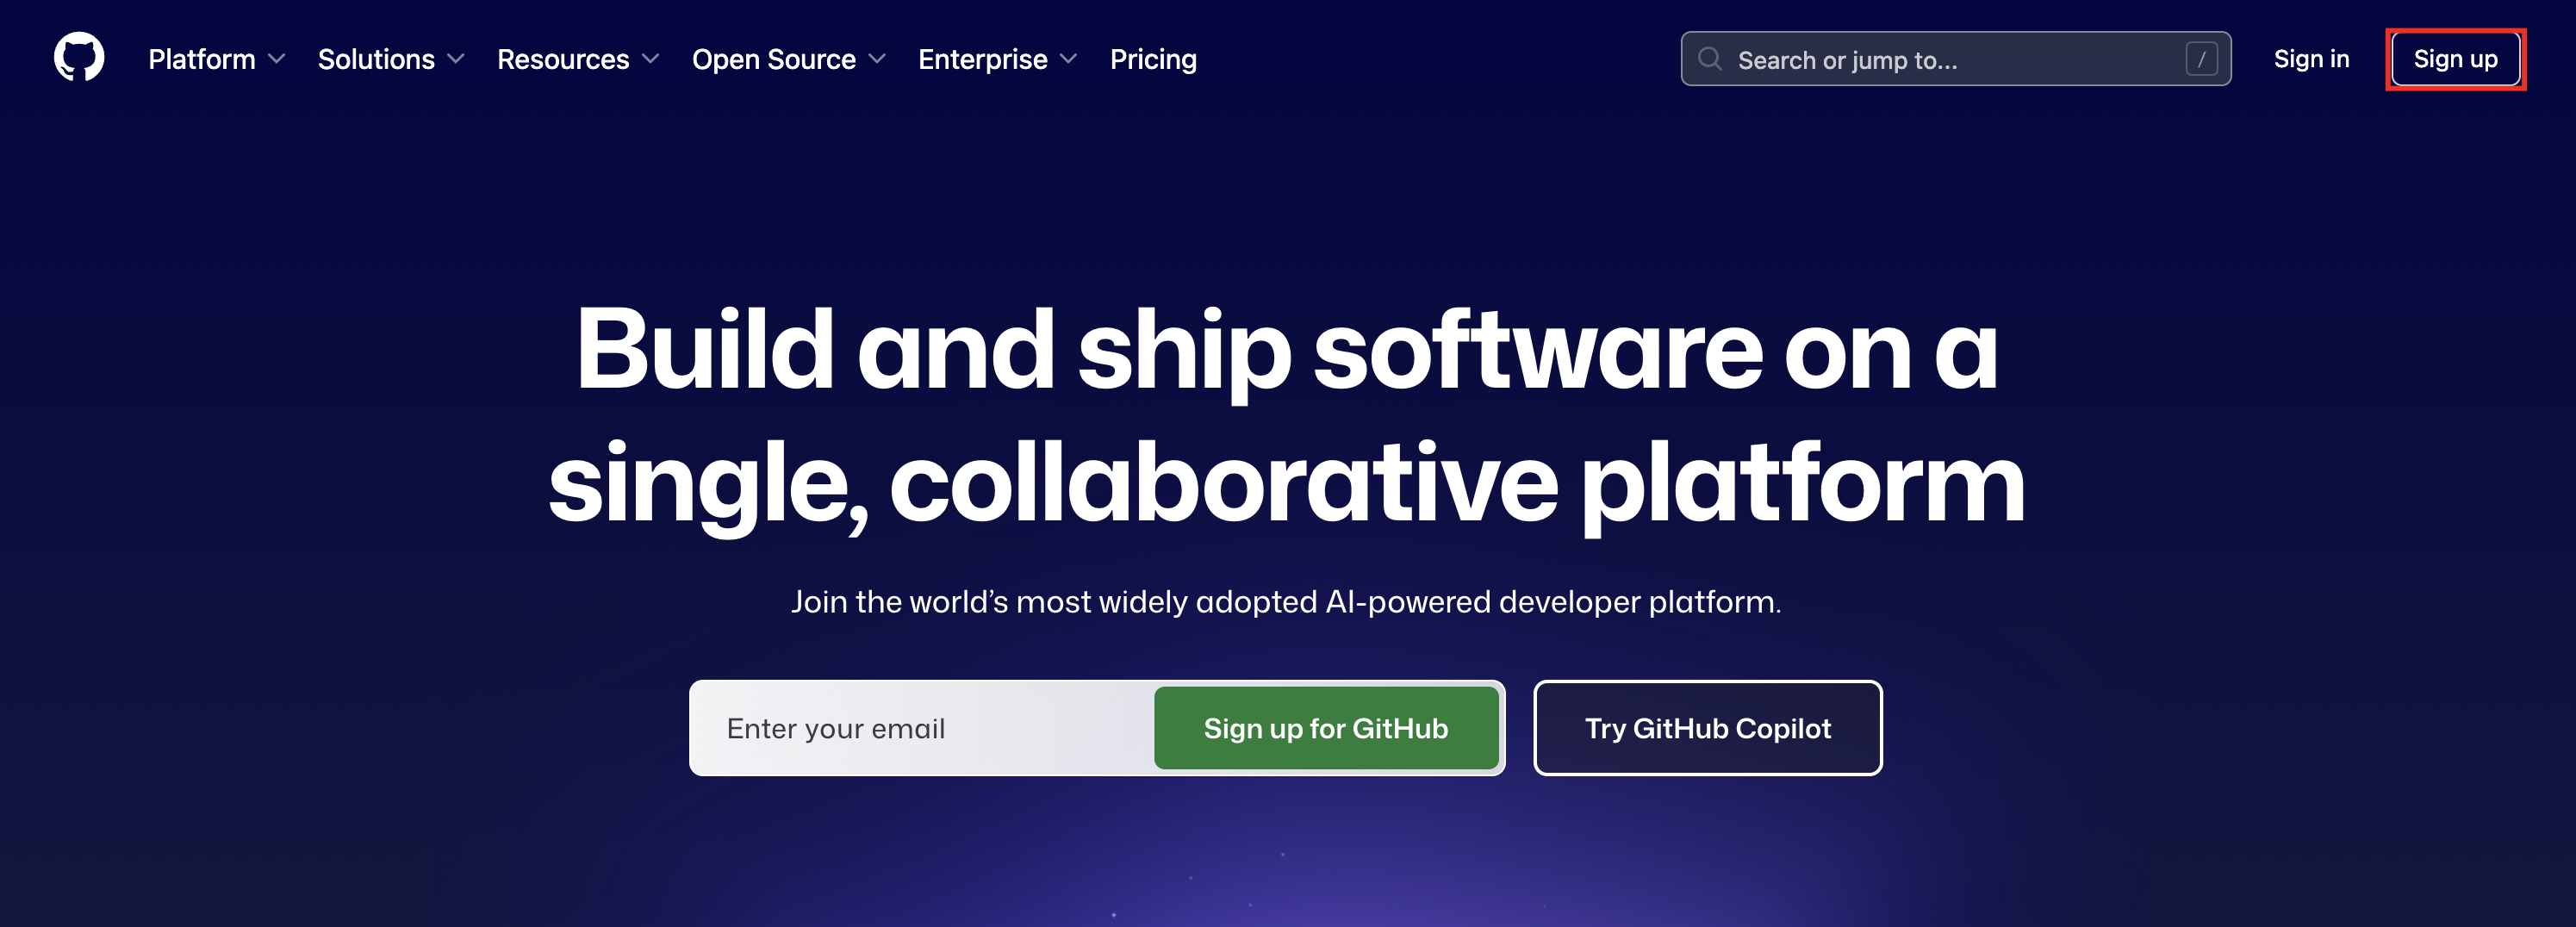
\includegraphics[width=0.6\textwidth]{imgs/tutorial_criar_conta_github/1_sign_up.png}
\caption{Botão "Sign up".}
\label{fig:sign_up}
\end{figure}

    \item \textbf{Informe seu e-mail, nome de usuário desejado e senha e crie sua conta.}  
    Digite um endereço de e-mail válido. Você receberá um código de verificação neste e-mail. Escolha um nome de usuário único, que será seu identificador público no GitHub. Crie uma senha forte. Clique no botão "Create account" para continuar, como mostrado na Figura \ref{fig:create_account}.
    
\begin{figure}[H]
\centering
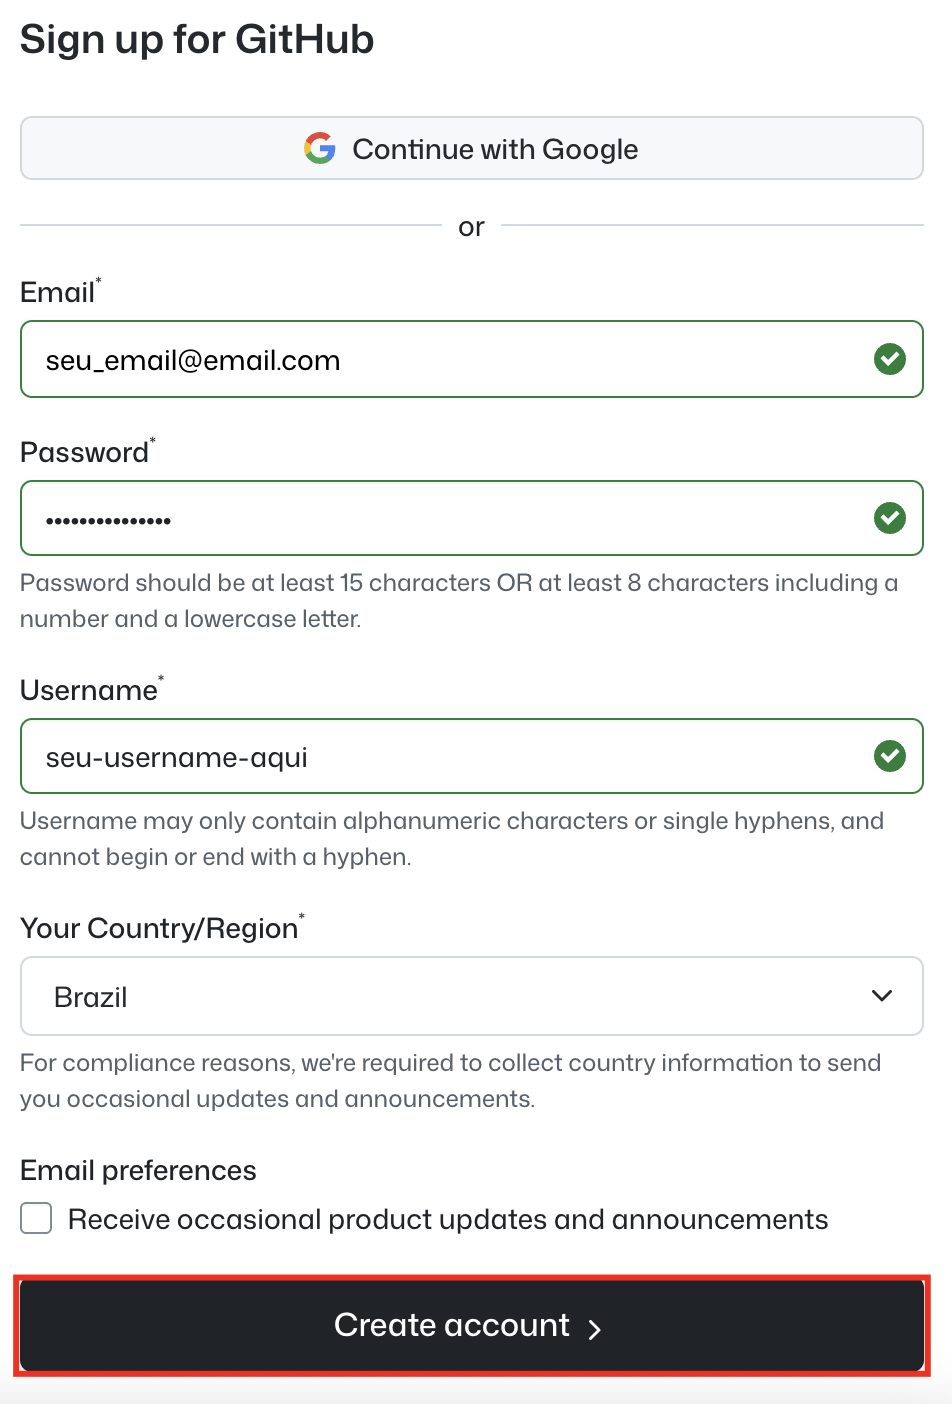
\includegraphics[width=0.5\textwidth]{imgs/tutorial_criar_conta_github/2_create_account.png}
\caption{Informações da conta e botão "Create account".}
\label{fig:create_account}
\end{figure}


    \item \textbf{Informe o código enviado ao e-mail.}  
    Caso necessário, informe o código enviado ao seu e-mail.

    \item \textbf{Configuração inicial:}  
    Após o cadastro e primeira conexão na sua conta, você pode adicionar uma foto de perfil, preencher sua bio e configurar autenticação em dois fatores para maior segurança. Para isso, primeiro clique na sua foto de perfil, no canto direito superior da página inicial, como mostrado na Figura \ref{fig:profile_image}.

\begin{figure}[H]
\centering
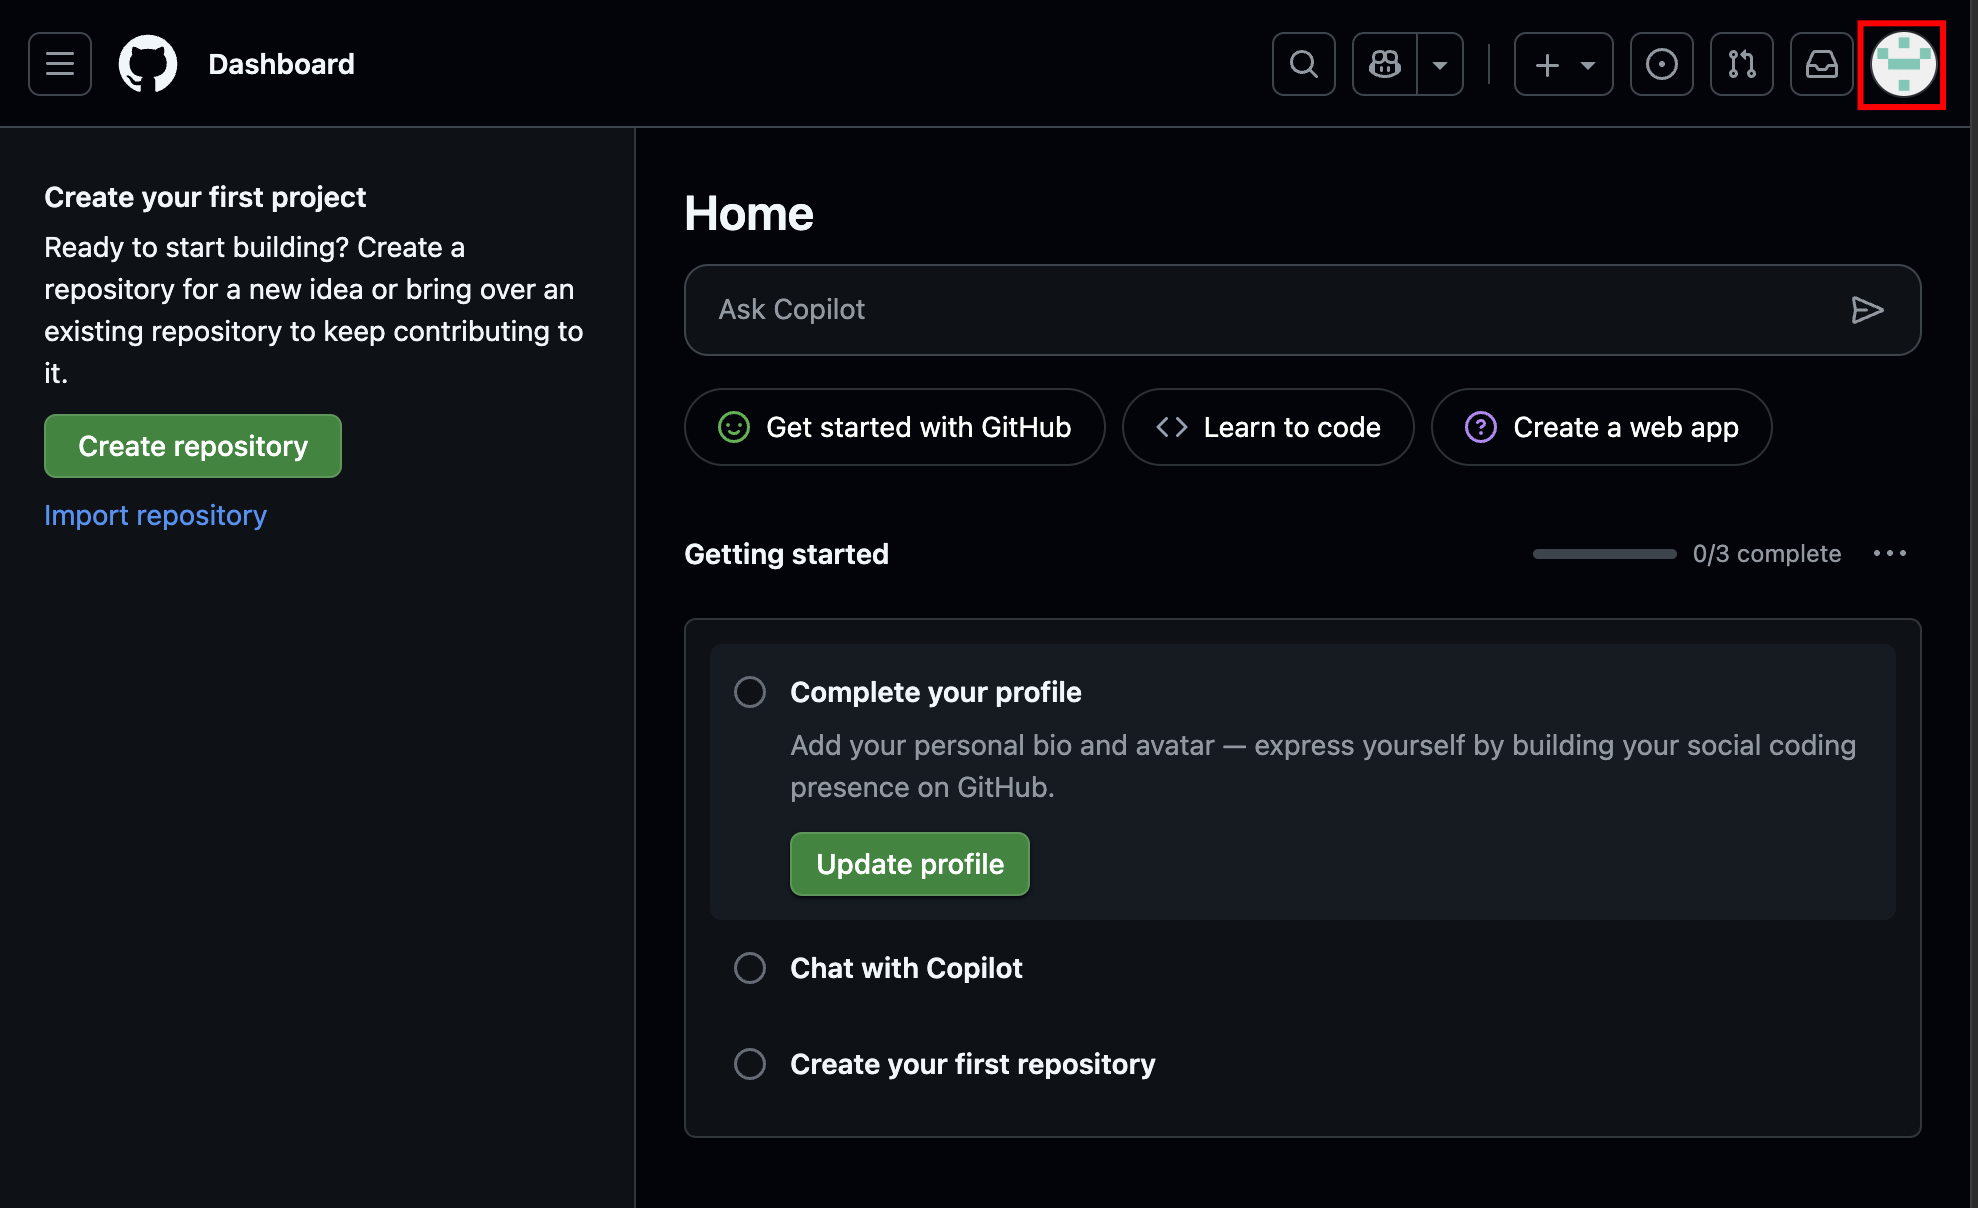
\includegraphics[width=0.6\textwidth]{imgs/tutorial_criar_conta_github/3_profile_image.png}
\caption{Foto de perfil no Github.}
\label{fig:profile_image}
\end{figure}

    \item \textbf{Navegue até as configurações do perfil:}
    Clique na aba "Profile", como mostrado na Figura \ref{fig:profile}. 
    
\begin{figure}[H]
\centering
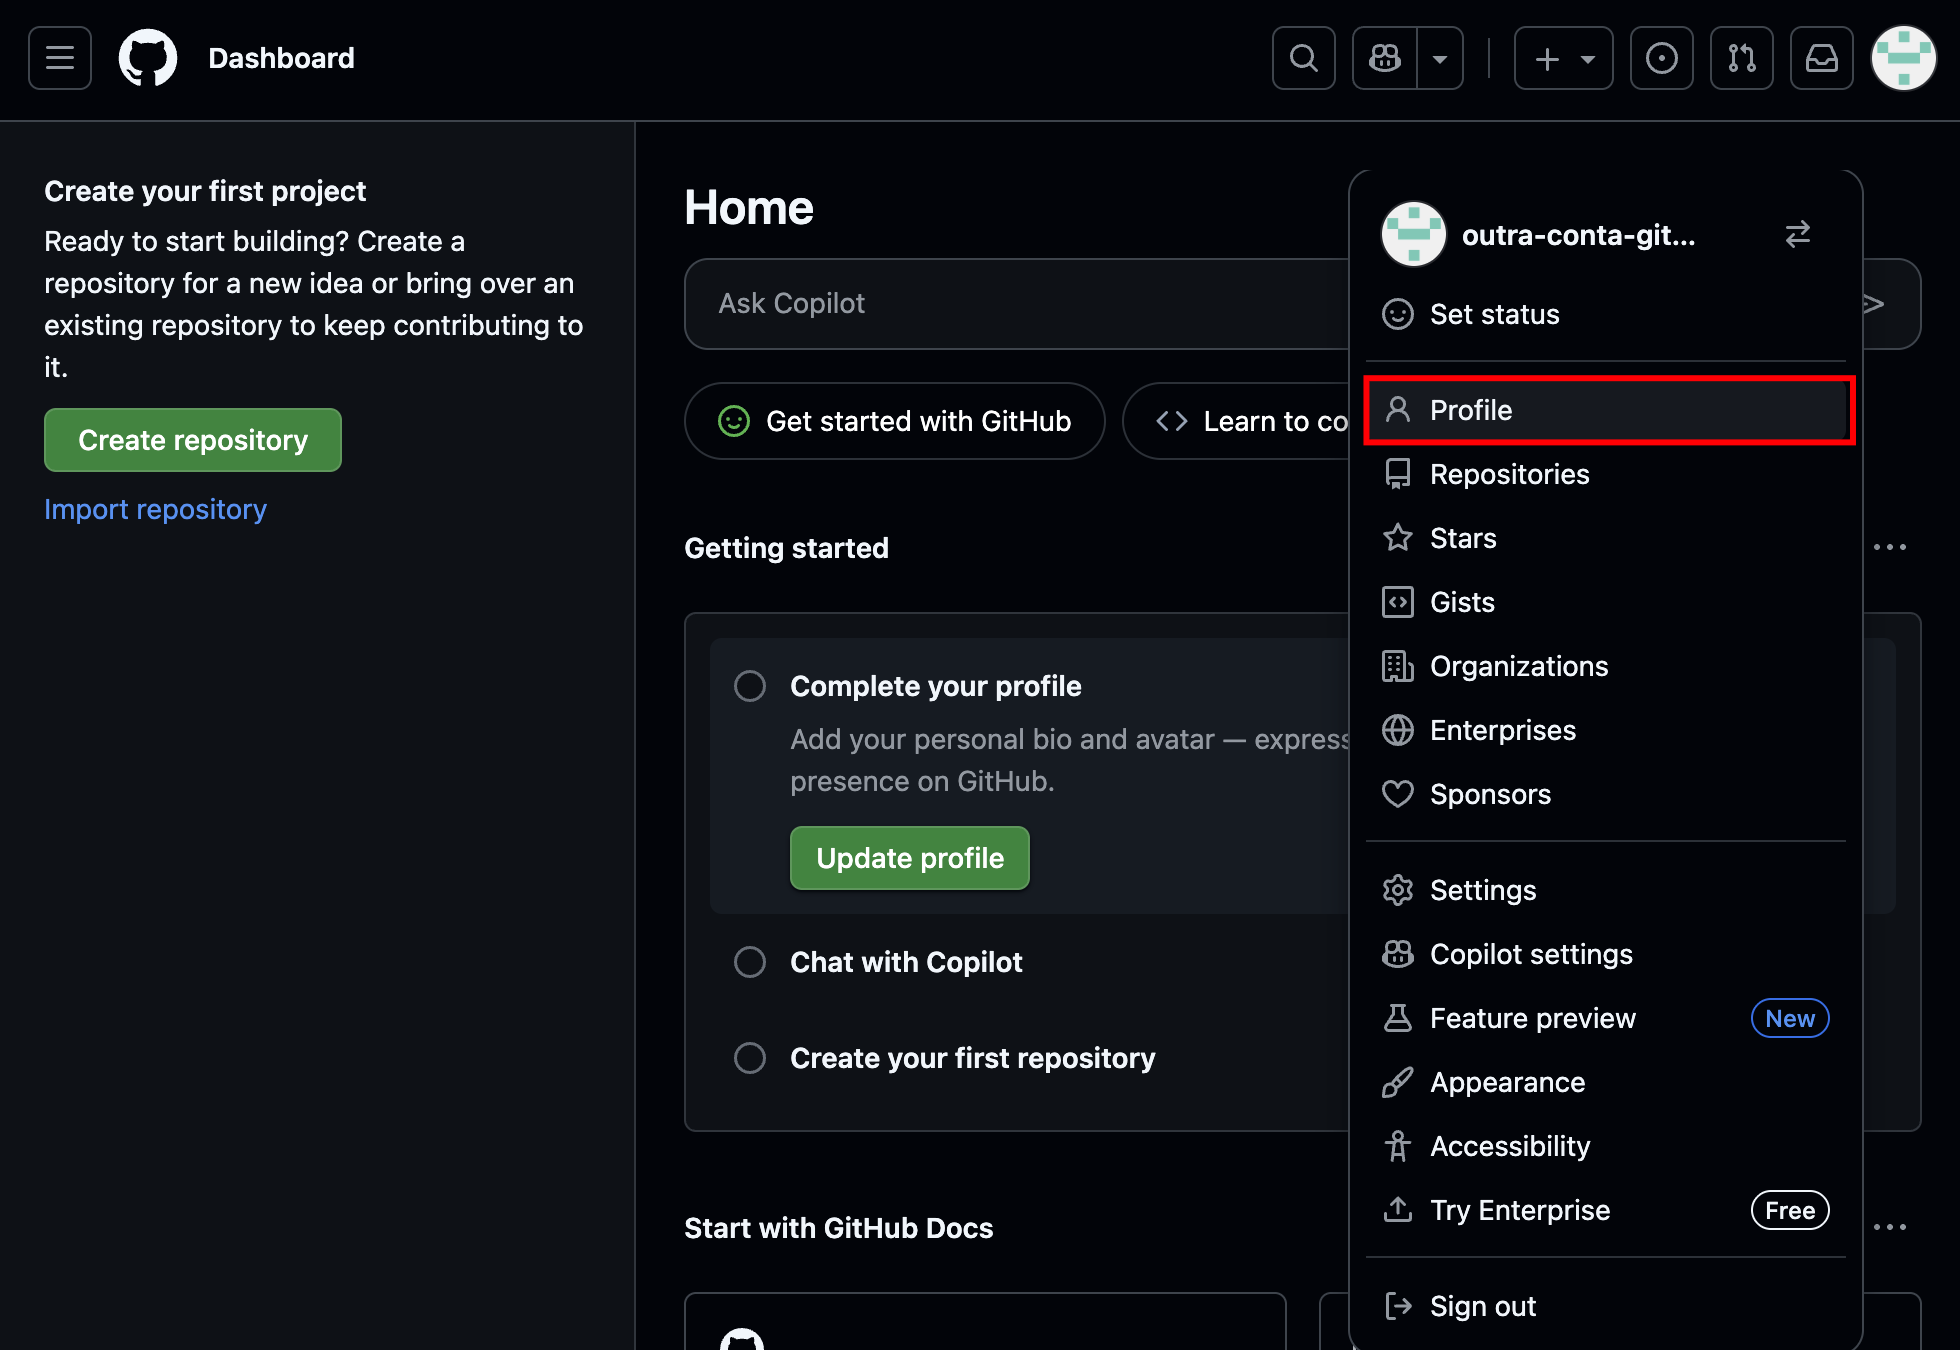
\includegraphics[width=0.6\textwidth]{imgs/tutorial_criar_conta_github/4_profile.png}
\caption{Aba "Profile" no Github.}
\label{fig:profile}
\end{figure}

Na sequência, clique em "Edit profile", como mostrado na Figura \ref{fig:edit_profile}. 

    \begin{figure}[H]
\centering
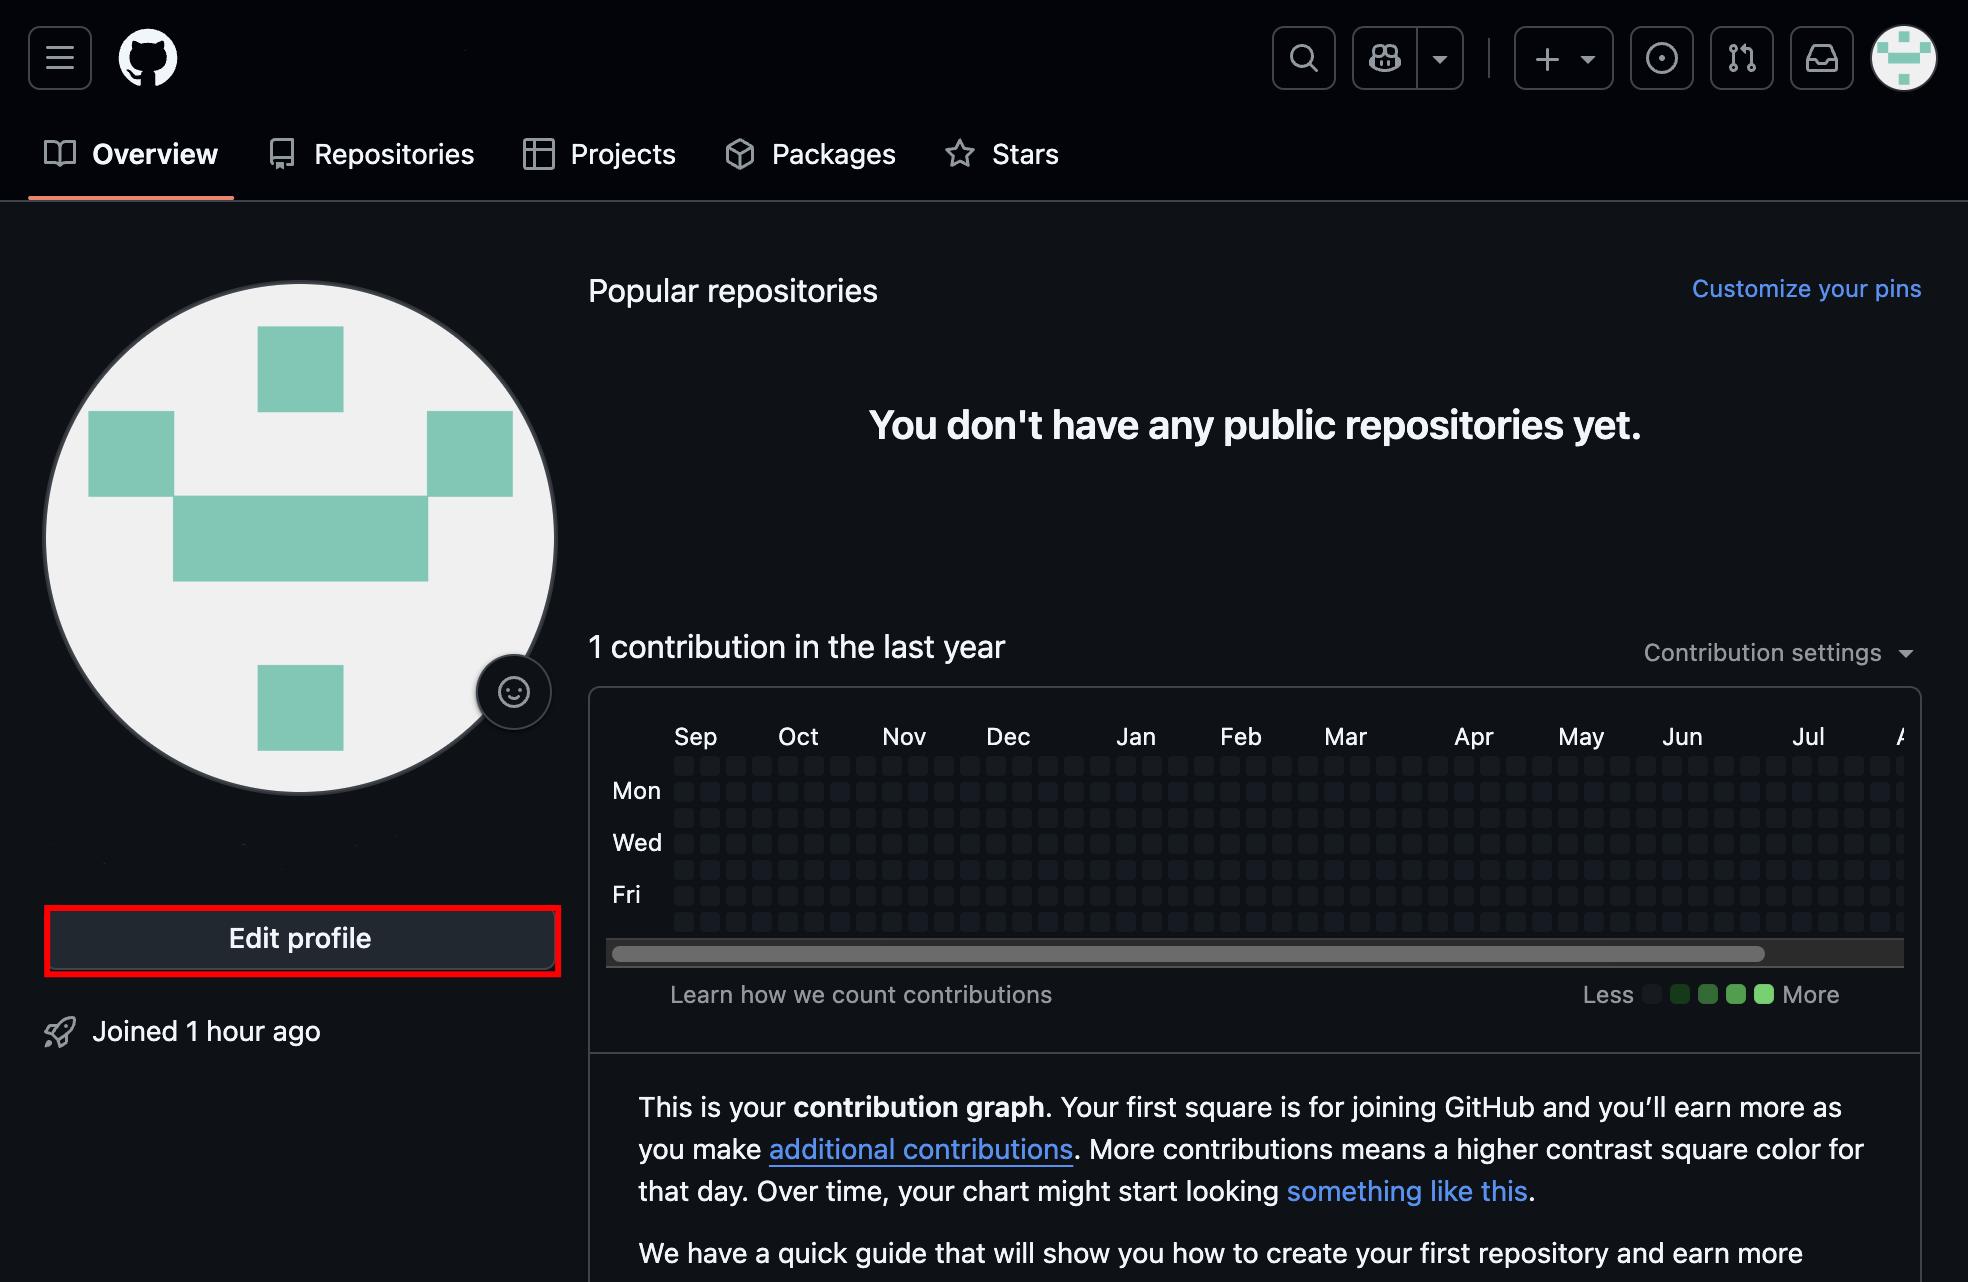
\includegraphics[width=0.6\textwidth]{imgs/tutorial_criar_conta_github/5_edit_profile.png}
\caption{Botão "Edit profile" no Github.}
\label{fig:edit_profile}
\end{figure}

Em seguida, edite as informações do seu perfil da maneira como desejar.

    \begin{figure}[H]
\centering
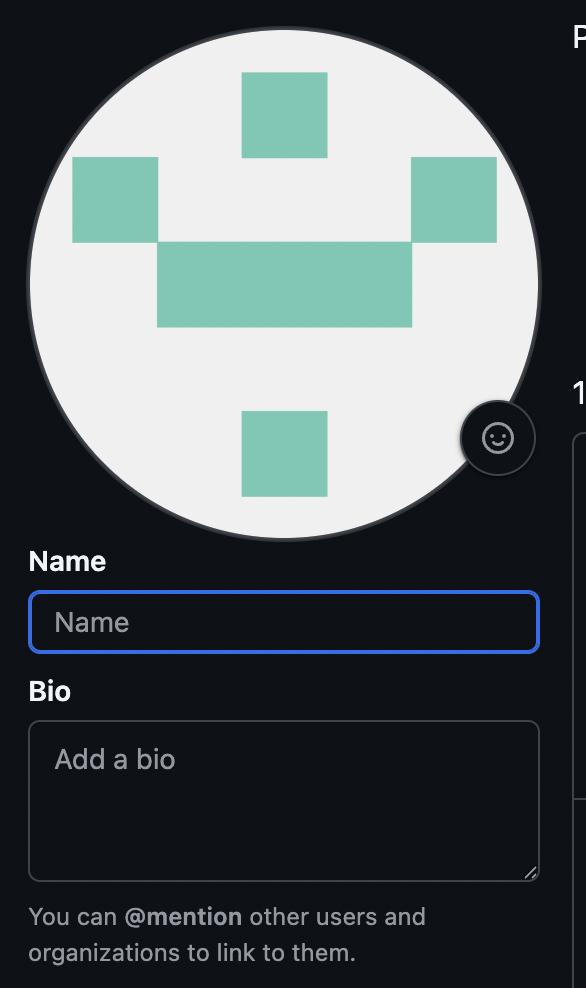
\includegraphics[width=0.4\textwidth]{imgs/tutorial_criar_conta_github/6_edit_info.png}
\caption{Configuração do seu perfil no Github.}
\label{fig:edit_info}
\end{figure}

\end{enumerate}

\subsection{Criação de uma chave SSH}
\label{cap:criacao_chave_ssh}

Para trabalhar com o GitHub, é possível realizar a comunicação com a plataforma de duas formas principais: HTTPS ou SSH.

A utilização de HTTPS é mais simples, pois não exige configuração inicial. No entanto, toda vez que for comunicar com o GitHub, é necessário informar usuário e senha ou um token de acesso.

Já o uso de SSH permite uma conexão mais prática e segura. Ao gerar uma chave SSH e adicioná-la à sua conta do GitHub, a autenticação passa a ser feita de forma automática, sem a necessidade de informar usuário e senha a cada comunicação. Essa abordagem é recomendada para quem utiliza o Git com frequência, pois agiliza o fluxo de trabalho e aumenta a segurança da comunicação.

Cada computador que se comunica com o GitHub precisa ter sua própria chave SSH. A chave é formada por duas partes: uma chave privada, que fica no computador e nunca deve ser compartilhada, e uma chave pública, que é adicionada à conta do GitHub. Assim, o GitHub reconhece o computador como autorizado a acessar os repositórios, sem precisar digitar usuário e senha a cada comunicação.

Para gerar uma chave SSH, no VS Code, abra o terminal integrado (\texttt{Ctrl + \`}) e siga os passos abaixo para gerar a chave SSH:

\begin{enumerate}
    \item Digite o comando abaixo, substituindo seu e-mail pelo utilizado no GitHub:
    \begin{lstlisting}[style=shellstyle]
ssh-keygen -t ed25519 -C "seu-email@exemplo.com"
    \end{lstlisting}
    \item Pressione \texttt{Enter} para aceitar o local padrão onde a chave será salva.
    \item Opcionalmente, digite uma senha para proteger a chave privada ou pressione \texttt{Enter} para deixar em branco.
    \item A chave será criada em duas partes: a chave privada (\texttt{id\_ed25519}) e a chave pública (\texttt{id\_ed25519.pub}).
\end{enumerate}

A chave privada deve permanecer no computador e nunca ser compartilhada. A chave pública será usada para configurar o acesso ao GitHub.

Para adicionar sua chave pública ao Github, primeiramente, copie os conteúdos do arquivo \texttt{id\_ed25519.pub}. Para fazer isso, use:

\begin{lstlisting}[style=shellstyle]
cat ~/.ssh/id_ed25519.pub
\end{lstlisting}

O comando \texttt{cat} mostra no terminal os conteúdos de um arquivo. Copie a chave mostrada. Ela deve ter o seguinte formato:

\begin{lstlisting}[style=shellstyle]
ssh-ed25519 <caracteres-aleatórios> seu-email@exemplo.com
\end{lstlisting}

Na sequência, siga os seguintes passos:

\begin{itemize}
    \item \textbf{Clique novamente na sua foto de perfil no Github:}
    Desta vez, clique na aba "Settings".

\begin{figure}[H]
\centering
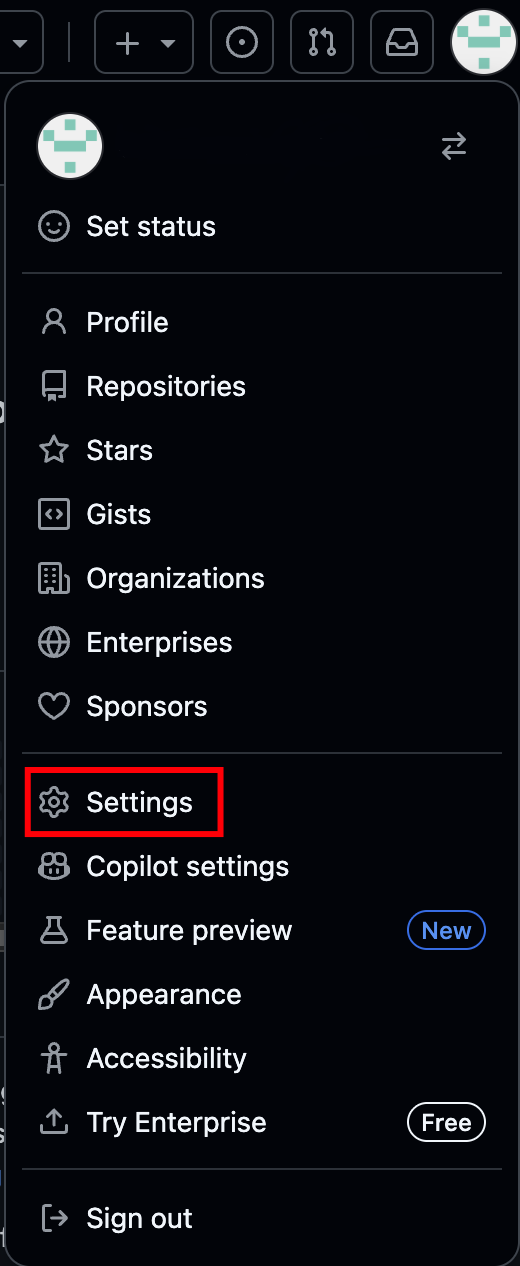
\includegraphics[width=0.3\textwidth]{imgs/tutorial_criar_conta_github/7_settings.png}
\label{fig:edit_info}
\caption{Aba "Settings" no Github.}
\end{figure}

\item \textbf{Clique na opção "SSH and GPG keys":}
Essa seção permite de configurar as chaves de acesso adicionados ao seu Github.

\begin{figure}[H]
\centering
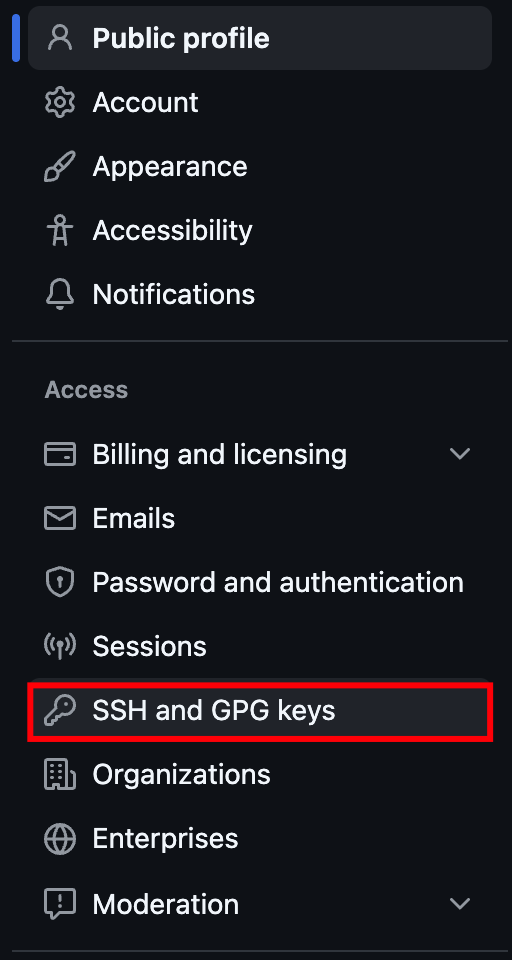
\includegraphics[width=0.4\textwidth]{imgs/tutorial_criar_conta_github/8_ssh_keys.png}
\label{fig:ssh_keys}
\caption{Opção "SSH and GPG keys".}
\end{figure}

\item \textbf{Clique em "New SSH key":}
Clique nesse botão para adicionar uma nova chave SSH.

    \begin{figure}[H]
\centering
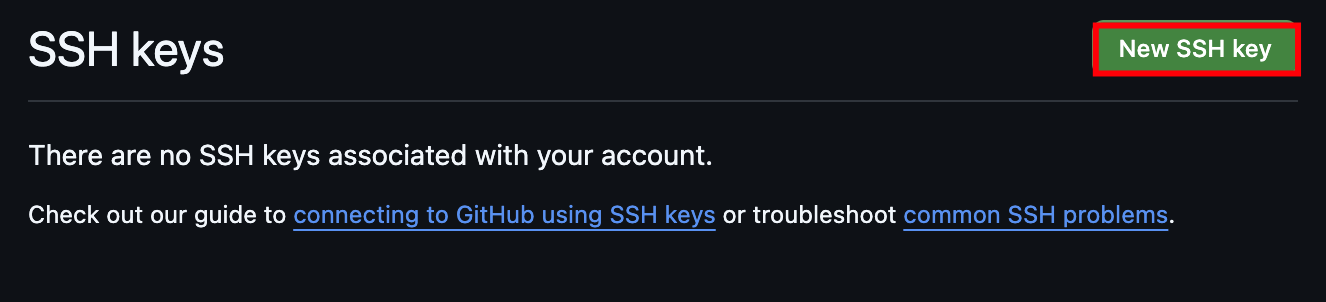
\includegraphics[width=0.8\textwidth]{imgs/tutorial_criar_conta_github/9_new_ssh_key.png}
\label{fig:ssh_keys}
\caption{Botão "New SSH key".}
\end{figure}

\item \textbf{Adicione as informações:}
    Coloque um nome que identifique a chave SSH que você está adicionando. Lembre-se que uma chave de acesso por computador é necessária. Nomes descritivos são úteis, como "Laptop" ou "Computador de casa". Cole a sua chave SSH pública. Clique em "Add SSH key" para adicionar a chave.

    \begin{figure}[H]
\centering
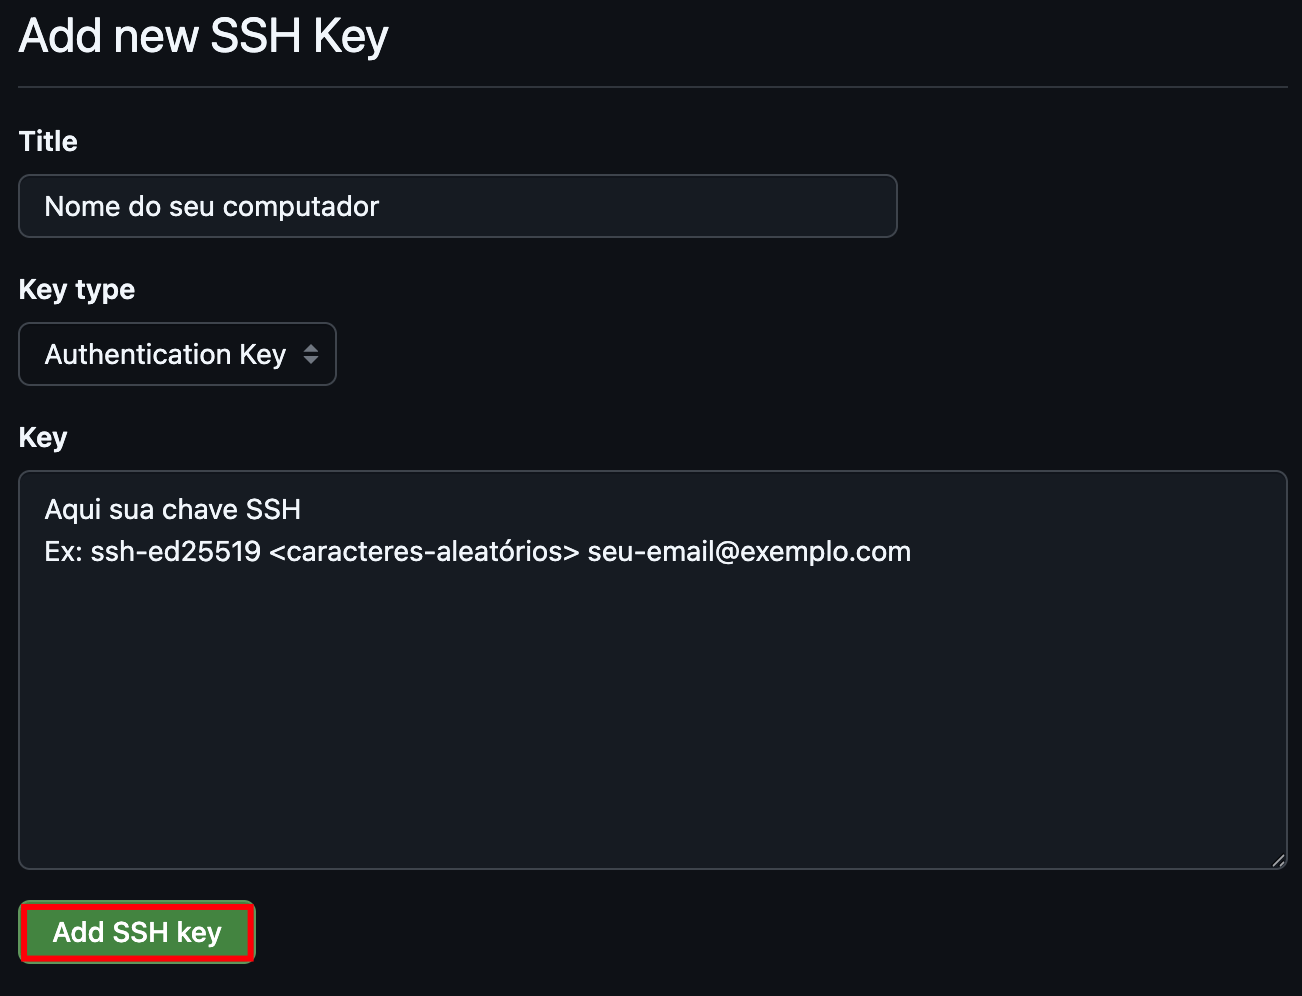
\includegraphics[width=0.5\textwidth]{imgs/tutorial_criar_conta_github/10_add_ssh_key.png}
\label{fig:ssh_keys}
\caption{Botão "Add SSH key".}
\end{figure}

\end{itemize}



